\documentclass[14pt,a4paper]{report}  %紙張設定
\usepackage{xeCJK}%中文字體模組
\setCJKmainfont{標楷體} %中文字體
\newfontfamily\sectionef{Times New Roman}%設定英文字體
\usepackage{amsmath,amssymb}%數學公式、符號
\usepackage{graphicx, subfig}%圖形
\usepackage{graphicx, subfig}%圖片模組
\usepackage{type1cm} %調整字體絕對大小
\usepackage{textpos} %設定文字絕對位置
\usepackage[top=2.5truecm,bottom=2.5truecm,
left=3truecm,right=2.5truecm]{geometry}
\usepackage{titlesec} %目錄標題設定模組
\usepackage{titletoc} %目錄內容設定模組
\usepackage{CJK} %中文模組
\usepackage{CJKnumb} %中文數字模組
\usepackage{wallpaper} %浮水印
\usepackage{listings} %能加入程式碼
\lstset{language=python}
\usepackage{hyperref} %引用url連結
\usepackage{graphicx} %插入圖片
\usepackage{fontawesome5} %引用icon
\lstset{language=Python, %設定語言
		basicstyle=\footnotesize, 
		frame=lines,
		caption={Python code}, %設定capion
		label={lst:example} %設定label
}
\graphicspath{{./圖片/}} %圖片預設讀取路徑
 %=------------------更改標題內容----------------------=%
\titleformat{\chapter}[hang]{\sectionef\fontsize{20pt}{2.5pt}\bfseries}{\Large 第\CJKnumber{\thechapter}章}{1em}{}[]
\titleformat{\section}[hang]{\sectionef\fontsize{18pt}{2.5pt}\bfseries}{{\thesection}}{1em}{}[]
\titleformat{\subsection}[hang]{\sectionef\fontsize{18pt}{2.5pt}\bfseries}{{\thesubsection}}{1em}{}[]
%=------------------更改目錄內容-----------------------=%
\titlecontents{chapter}[11mm]{}{\sectionef\fontsize{18pt}{2.5pt}\bfseries\makebox[3.5em][l]
{第\CJKnumber{\thecontentslabel}章}}{}{\titlerule*[0.7pc]{.}\contentspage}
\titlecontents{section}[18mm]{}{\sectionef\LARGE\makebox[1.5em][l]
{\thecontentslabel}}{}{\titlerule*[0.7pc]{.}\contentspage}
\titlecontents{subsection}[4em]{}{\sectionef\Large\makebox[2em][l]{{\thecontentslabel}}}{}{\titlerule*[0.7pc]{.}\contentspage}
%=----------------------標題-------------------------=%             
\begin{document} %文件
\begin{titlepage}%開頭
\begin{center}   %標題  
\makebox[1.5\width][s]
{\fontsize{24pt}{2.5pt}國立虎尾科技大學}\\[18pt]
\makebox[1.5\width][s]
{\fontsize{24pt}{2.5pt}機械設計工程系}\\[18pt]
\makebox[1.5\width][s]
{\fontsize{24pt}{2.5pt}專題製作報告}\\[18pt]
%設定文字盒子 [方框寬度的1.5倍寬][對其方式為文字平均分分布於方框中]\\距離下方18pt
\vspace{3em} %下移
\fontsize{30pt}{1pt}\textbf{強化學習在機電系統設計與控制\\
\vspace{1em}中之應用}\\
\vspace{4em}
\sectionef\fontsize{30pt}{1em}\textbf
{
\vspace{0.5em}
Application of reinforcement
 \vspace{0.5em} 
 learning in design and control of mechatronic systems}
 \vspace{2em}
%=---------------------參與人員-----------------------=%             
\end{center}
\begin{flushleft}
\begin{LARGE}
\hspace{32mm}\makebox[5cm][s]
{指導教授:\quad 嚴\quad 家\quad 銘\quad 老\quad 師}\\[6pt]
\hspace{32mm}\makebox[5cm][s]
{班\qquad 級:\quad 四\quad 設\quad 三\quad 甲}\\[6pt]
\hspace{32mm}\makebox[5cm][s]
{學\qquad 生:\quad 李\quad 正\quad 揚\quad(40723110)}
\\[6pt]
\hspace{32mm}\makebox[5cm][s]
{\hspace{36.5mm}林\quad 于\quad 哲\quad(40723115)}\\[6pt]
\hspace{32mm}\makebox[5cm][s]
{\hspace{36.5mm}黃\quad 奕\quad 慶\quad(40723138)}\\[6pt]
\hspace{32mm}\makebox[5cm][s]
{\hspace{36.5mm}鄭\quad 博\quad 鴻\quad(40723148)}\\[6pt]
\hspace{32mm}\makebox[5cm][s]
{\hspace{36.5mm}簡\quad 國\quad 龍\quad(40723150)}\\[6pt]
%設定文字盒子[寬度為5cm][對其方式為文字平均分分布於方框中]空白距離{36.5mm}\空白1em
\end{LARGE}
\end{flushleft}
\vspace{3em}
\fontsize{18pt}{2}\centerline{\makebox[\width][s]
{中華民國\hspace{3em} 
110 \quad 年\quad 3\quad 月}}
\end{titlepage}
\newpage
%=------------------------摘要-----------------------=%
\pagenumbering{roman}
\clearpage
\addcontentsline{toc}{chapter}{摘\quad 要} %將摘要加入目錄
\begin{center}
\LARGE\textbf{摘要}\\
\begin{flushleft}
\fontsize{14pt}{2.5pt}\hspace{12pt} 產業中需要加速許多工法的演算,以達到最佳化,但不能以實體一直測試不同方法,成本與時間不允許,便可以利用許多感測器觀測數值,以類神經網路運算,在虛擬環境架設結構,遠端控制、更改數值。\\
\vspace{1em}
\sectionef\hspace{12pt} 此專題是利用現成裝置冰球台,設置對應虛擬模擬環境,減少現實模擬參數設置、成本,再加入類神經網路之中的 Policy gradient與Reinforcement Learning,訓練冰球達到對應最佳化。
\end{flushleft}
\begin{center}
\fontsize{14pt}{2.5pt}關鍵字:\sectionef Policy gradient、虛擬環境架設結構、Reinforcement Learning
\end{center}
\newpage
%=------------------------誌謝----------------------=%
\addcontentsline{toc}{chapter}{誌\quad 謝}
\centerline\LARGE\textbf{誌謝}\\
\begin{flushleft}
\fontsize{14pt}{2.5pt}\hspace{12pt}致謝內容
\end{flushleft}
\newpage
%=------------------------目錄----------------------=%
\renewcommand{\contentsname}{\centerline{\fontsize{18pt}{\baselineskip}\selectfont\textbf{目\quad 錄}}}
\tableofcontents  %目錄產生
\newpage
%=------------------圖表目錄產生----------------------=%
\renewcommand{\listfigurename}{\centerline{\fontsize{18pt}{\baselineskip}\selectfont\textbf{圖\quad 表\quad 目\quad 錄 }}}
\listoffigures
\newpage
\end{center}
%=-------------------------內容----------------------=%

\chapter{機器學習的訓練方法}
\pagenumbering{arabic} %設定頁號阿拉伯數字
\setcounter{page}{1}  %設定頁數
\fontsize{14pt}{2.5pt}\sectionef
\section{類神經網絡}
\qquad 類神經網路的概念來源是觀察人類的中樞神經系統而啟發的,類神經網路主要由多個節點組成,每個節點稱為神經元(neurons),神經元與神經元連結而形成的網路稱為神經網路。神經元主要又分成三層:輸入層(input layer)、隱藏層(hidden layer)和輸出層(output layer)。神經元會接收上一層的訊號,並經過啟動函數(activation function)計算並輸出至下一層神經元。神經網路輸入層的神經元負責接收訊號,透過隱藏層來運算,再傳遞到輸出層執行動作。由於每個神經元經過啟動函數的非線性計算,所以神經元傳出的數值也是非線性。神經元與神經元間連線在生物學稱為突觸(Synapse),在數學模型裡每個突觸都有權重(weights)。在既定框架下,調配權重值和啟動函數會使結果更接近預期。神經網路的架構指標為以下幾項:階層數、每層神經元個數、神經元連接方式、啟動函數的類型等。

神經訊號傳遞分為前饋(feed-forward)和回饋(backpropagation)。

前饋為傳遞經過啟動函數計算的數值。回饋則是修正權重和偏差(biases),以提高下次前饋計算的準確度。
\subsection{啟動函數}
\begin{itemize}
\item Sigmoid Function\\
\qquad An activation function.It is a key part of Nerual Network and it can be differentiable.It can make the Nenual Network unliner.\\
\begin{Large}$$\sigma(x)=\frac{1}{1+e^{-x}}$$ \end{Large}\\[6pt]
\begin{figure}[hbt!]
\begin{center}
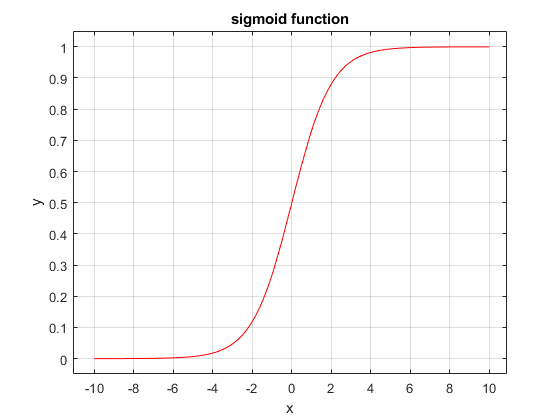
\includegraphics[scale=0.74]{sigmoid_function}
\caption{Sigmoid; 
from: \href{https://towardsdatascience.com/derivative-of-the-sigmoid-function-536880cf918e}{Toward Data Science}}
\end{center}
\end{figure}
%=----------SigmoidPrime Function----------=%
\item SigmoidPrime Function\\
\qquad It is an differential Sigmoid Funtion. It can reduce  error of gradient so it is some kind of loss function and Let's take a look the proof of SigmoidPrime\\
\begin{Large}$$\sigma(x)=\frac{1}{1+e^{-x}}$$ \end{Large}\\[6pt]
$$\sigma^{'}(x)=\frac{d}{dx}\sigma(x)=\frac{d}{dx}\frac{1}{1+e^{-x}}=\frac{d}{dx}(1+e^{-x})^{-1}$$\\[6pt]
$$-------------skip-------------$$\\[6pt]
Tip: find $f^{'}(x)$ if $f(x)=\frac{A}{B+Ce^{x}}$\\
Answer:\\
$$\frac{d}{dx}[\frac{1}{g(x)}]=\frac{1^{'}g(x)-1g^{'}(x)}{g(x)^2}=\frac{g^{'}(x)}{[g(x)]^2}$$\\
if $g(x)$=constant\\
$$\frac{d}{dx}[\frac{g(x)}{h(x)}]=\frac{g^{'}(x)h(x)-g(x)h^{'}(x)}{h(x)^2}= \frac{-kh^{'}(x)}{[h(x)]^2}$$\\
$$f^{'}(x)=\frac{-A[\frac{d}{dx}(B+Ce^x)]}{(B+Ce^x)^2}=\frac{-A(0+Ce^x)}{(B+Ce^x)^2}=\frac{-ACe^x}{(B+Ce^x)^2}$$\\[6pt]
$$-------------skip-------------$$\\[6pt]
Hence:\\
$$=-(1+e^{-x})^{-2}\frac{d}{dx}(1+e^{-x})=-(1+e^{-x})^{-2}[\frac{d}{dx}(1)+\frac{d}{dx}(e^{-x})]$$\\
$$=-(1+e^{-x})^{-2}[0+\frac{d}{dx}(e^{-x})]=-(1+e^{-x})^{-2}[\frac{d}{dx}(e^{-x})]=-(1+e^{-x})^{-2}[e^{-x}\frac{d}{dx}(-x)]$$\\
$$-(1+e^{-x})^{-2}[e^{-x}(-1)]=-(1+e^{-x})^{-2}(-e^{-x})=\frac{e^{-x}}{(1+e^{-x})^2}=\frac{1(e^{-x})}{(1+e^{-x})(1+e^{-x})}$$\\
$$=\frac{1}{1+e^{-x}}\frac{e^{-x}}{1+e^{-x}}=\frac{1}{1+e^{-x}}\frac{e^{-x}+1-1}{1+e^{-x}}=\frac{1}{1+e^{-x}}(\frac{1+e^{-x}}{1+e^{-x}}-\frac{1}{1+e^{-x}})$$\\[6pt]
\begin{Large}$$=\sigma(x)[1-\sigma(x)]$$\end{Large}\\
\begin{figure}[hbt!]
\begin{center}
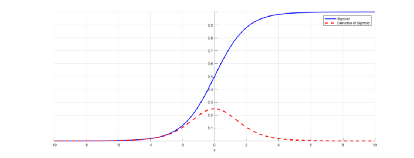
\includegraphics[scale=0.80]{sigmoidprime}
\caption{SigmoidPrime; from: \href{https://towardsdatascience.com/derivative-of-the-sigmoid-function-536880cf918e}{Toward Data Science}}
\end{center}
\end{figure}
%=----------Relu Function----------=%
\item Relu Function\\
\qquad This is the most commly used activation function in nerual network.It also can solve the Gradient Descent problem.
\begin{Large}$$f(x)=max(0,x)$$\end{Large}
$$if , x<0 , f(x)=0$$
$$else f(x)=x$$\\

%\begin{figure}[hbt!]
%\begin{center}
%\includegraphics[height=4.5cm]{relu}\\
%\caption{Relu; from : \href{https://www.kaggle.com/dansbecker/rectified-linear-units-relu-in-deep-learning}{\underline{kaggle}} }
%\end{center} 
%\end{figure}
%=----------Adam Function----------=%
\item Adam Function\\
\qquad Combine the advantage of Adagrad and RMSprop.The paper contained some very promising diagrams, showing huge performance gains in terms of speed of training but in some cases Adam actually finds worse solution than stochastic gradient descent. Let's take a look caculation prosess \\[6pt]
$$g_t=\delta_{\theta}f(\theta)$$\\
First moment exponentially moving averages : $m_t =\beta(m_{t-1})+(1-\beta_1)(\nabla{w_t})$\\[6pt]
$\hat m_t=\frac{m_t}{1-\beta_1^t}$\\[6pt]
Second moment exponentially moving averages :$v_t=\beta_2(v_t-1)+(1-\beta_2)(\nabla{w_t})^2$\\[6pt]
$\hat{v_t}=\frac{v_t}{1-\beta_2^t}$\\[6pt]
Hence,Adam Function:\\[6pt]
\begin{Large}$$\omega_{t-1}=\omega_t-\frac{\eta}{\sqrt{\hat{v_t}-\epsilon}}\hat{m_t}$$\end{Large}
%=----------Mean Squared Error----------=%
\item Mean Squared Error\\
\qquad It tells you how close a regression lines to a set of points.It does this by taking the distances from the points to the regression line (these distances are the “errors”) and squaring them.The squaring is necessary to remove any negative signs. It also gives more weight to larger differences.
(\href{https://www.statisticshowto.com/mean-squared-error/}{\underline{Extracted from here)}}.\\[6pt]
\begin{figure}
\center
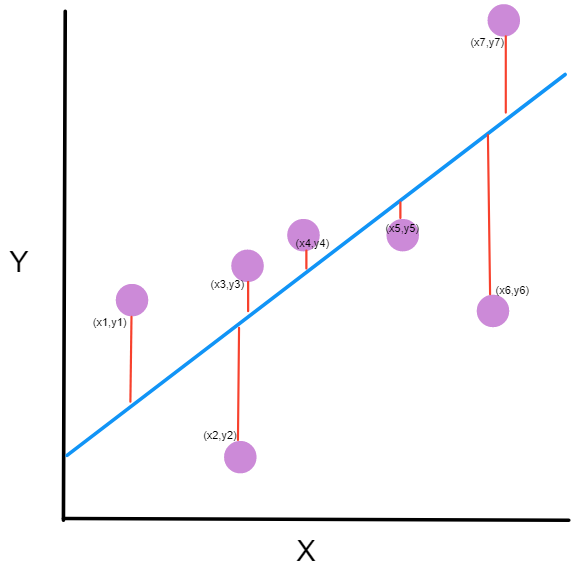
\includegraphics[height=7cm]{MSE}
\caption{regression line}
\end{figure}

regression line :It is a line of the minimize distance of data points. \\
n : number of data points\\
$y_i$ :  observed values\\
$\hat{y_i}$ : predicted values\\
\begin{Large}
$$MSE=\frac{1}{n} \sum_{i=1}^n(y_i-\overline{y} _i)^2$$
\end{Large}\\[6pt]
\newpage
\end{itemize}
\section{深度學習}
\newpage
\section{強化學習}
%=----------deep learning 會在此時崛起?----------------=%
\begin{itemize}

\item Deep learning 會在此時崛起?\\
\qquad Four major trends in scientific computing have become increasingly important for deep learning.\\

(1)\quad 支援張量運算程式語言與程式庫的崛起\\ First, starting in the 1960s, the development of domain specific languages such as APL, MATLAB, R and Julia, turned multidimensional arrays (often referred to as tensors) into first-class objects supported by a comprehensive set of mathematical primitives (or operators) to manipulate them.\\
Separately, libraries such as NumPy, Torch, Eigen and Lush made array-based programming productive in general purpose languages such as Python, Lisp, C++ and Lua.\\

(2)\quad 自動求導數套件的開發\\ Second, the development of automatic differentiation made it possible to fully automate the daunting labor of computing derivatives. This made it significantly easier to experiment with different machine learning approaches while still allowing for efficient gradient based optimization. The autograd package popularized the use of this technique for NumPy arrays, and similar approaches are used in frameworks such as Chainer, DyNet, Lush, Torch, Jax and Flux.jl.\\

(3)\quad 自由開源軟體的普及\\ Third, with the advent of the free software movement, the scientific community moved away from closed proprietary software such as Matlab, and towards the open-source Python ecosystem with packages like NumPy, SciPy, and Pandas. This fulfilled most of the numerical analysis needs of researchers while allowing them to take advantage of a vast repository of librariesto handle dataset preprocessing, statistical analysis, plotting, and more.\\
Moreover, the openness, interoperability, and flexibility of free software fostered the development of vibrant communities that could quickly address new or changing needs by extending the existing functionality of a library or if needed by developing and releasing brand new ones. While there is a rich offering of open-source software for neural networks in languages other than Python, starting with Lush in Lisp, Torch in C++, Objective-C and Lua, EBLearn in C++, Caffe in C++, the network effects of a large ecosystem such as Python made it an essential skill to jumpstart one’s research. Hence, since 2014,most deep learning frameworks converged on a Python interface as an essential feature.\\

(4)\quad 多核 GPU 運算的發展 \\ Finally, the availability and commoditization of general-purpose massively parallel hardware such as GPUs provided the computing power required by deep learning methods. Specialized librariessuch as cuDNN, along with a body of academic work (such as Andrew Lavin. maxdnn: An efficient convolution kernel for deep learning with maxwell gpus,January 2015 and Andrew Lavin and Scott Gray. Fast algorithms for convolutional neural networks.2016 IEEEConference on Computer Vision and Pattern Recognition (CVPR), pages 4013–4021, 2016), produced aset of high-performance reusable deep learning kernels that enabled frameworks such as Caffe,Torch7, or TensorFlow to take advantage of these hardware accelerators.\\
%=----------What is Reinforcement Learning?------------=%
\item What is Reinforcement Learning?\\
強化學習是通過agent與已知或未知的環境持互動,不斷適應與學習,得到的回饋可能是正面,也就是reward,如果得到負面,那就是punishments。考慮到agent與環境互動,我們就能決定要執行哪個動作。簡而言之,強化學習是建立在reward與punishments上。\\[6pt]
\\
\begin{large}
\textbf{The key point of Reinforcement Learning:}
\end{large}\\
\begin{itemize}
\item It differs from normal Machine Learning, as we do not look at
training datasets. 
\end{itemize}
\begin{itemize}
\item Interaction happens not with data but with environments,
through which we depict real-world scenarios
\end{itemize}
\begin{itemize}
\item As Reinforcement Learning is based on environments, many
parameters come in to play. It takes lots of information to learn
and act accordingly.
\end{itemize}
\begin{itemize}
\item Environments in Reinforcement Learning are real-world
scenarios that might be 2D or 3D simulated worlds or gamebased scenarios.
\end{itemize}
\begin{itemize}
\item Reinforcement Learning is broader in a sense because the
environments can be large in scale and there might be a lot of
factors associated with them.
\end{itemize}
\begin{itemize}
\item The objective of Reinforcement Learning is to reach a goal.
\end{itemize}
\begin{itemize}
\item Rewards in Reinforcement Learning are obtained from the
environment.
\end{itemize}
%=----------Faces of Reinforcement Learning---------------=%
\item Faces of Reinforcement Learning\\
\begin{figure}[hbt!]
\begin{center}
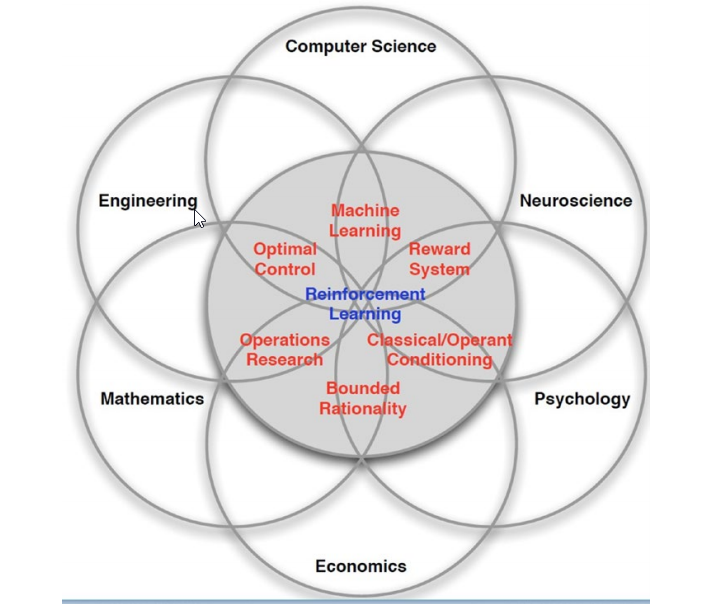
\includegraphics[scale=0.74]{Faces_of_Reinforcement_Learning}
\caption{Venn diagram; }%from: \href{file:///H:/201906_fall/data/tmp/project2020-1/downloads/reinforcement_learning/2018_Book_ReinforcementLearning.pdf}{All the faces of Reinforcement Learning}
\end{center}
\end{figure}
%=--------The Flow of Reinforcement Learning------------=%
\item The Flow of Reinforcement Learning\\
\begin{figure}[hbt!]
\begin{center}
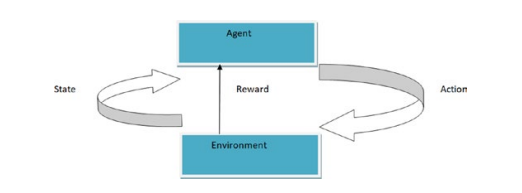
\includegraphics[scale=0.74]{The_Flow_of_Reinforcement_Learning}
\caption{RL structur}
\end{center}
\end{figure}
\begin{large}
\textbf{The key points of consideration:}
\end{large}\\
\begin{itemize}
\item The Reinforcement Learning cycle works in an interconnected. 
\end{itemize}

\begin{itemize}
\item The distinct communication happens with rewards in mind.
\end{itemize}
\begin{itemize}
\item There is distinct communication between the agent and the 
environment. 
 
\end{itemize}
\begin{itemize}
\item The object or robot moves from one state to another. 
 
\end{itemize}
\begin{itemize}
\item An action is taken to move from one state to another 
\end{itemize}

\begin{figure}[hbt!]
\begin{center}
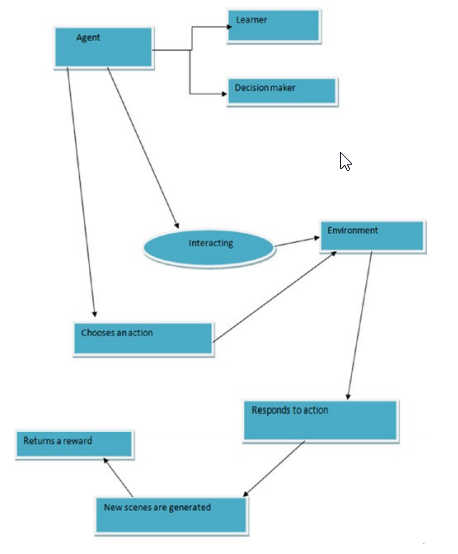
\includegraphics[scale=0.74]{The_entire_interaction_process}
\caption{The entire interaction process; }%from: \href{file:///H:/201906_fall/data/tmp/project2020-1/downloads/reinforcement_learning/2018_Book_ReinforcementLearning.pdf}{All the faces of Reinforcement Learning}
\end{center}
\end{figure}
The agent is also a decision maker because it tries to take an action that will get it the 
maximum reward.\\
When the agent starts interacting with the environment, it can choose an action and 
respond accordingly.
From then on, new scenes are created. When the agent changes from one place to 
another in an environment, every change results in some kind of modification. These 
changes are depicted as scenes. The transition that happens in each step helps the agent 
solve the Reinforcement Learning problem more effectively\\
\begin{figure}[hbt!]
\begin{center}
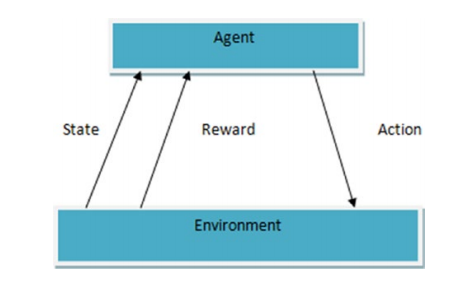
\includegraphics[scale=0.74]{Scenario_of_state_changes}
\caption{The entire interaction process; }%from: \href{file:///H:/201906_fall/data/tmp/project2020-1/downloads/reinforcement_learning/2018_Book_ReinforcementLearning.pdf}{All the faces of Reinforcement Learning}
\end{center}
\end{figure}
%=----Different Terms in Reinforcement Learning----------=%
\item Different Terms in Reinforcement Learning\\
There are two constants that are important in this case—gamma (γ) and lambda (λ)\\[10pt]
Gamma is used in each state transition and is a constant value at each state change. 
Gamma allows you to give information about the type of reward you will be getting in 
every state. 
Gamma (γ) is called a discount 
factor and it determines what future reward types we get:\\
\begin{itemize}
\item A gamma value of 0 means the reward is associated with the 
current state only.
\end{itemize}

\begin{itemize}
\item A gamma value of 1 means that the reward is long-term.
\end{itemize}
Lambda is generally used when we are dealing with temporal difference problems. It is 
more involved with predictions in successive states.
Increasing values of lambda in each state shows that our algorithm is learning fast. 
The faster algorithm yields better results when using Reinforcement Learning techniques.
As you’ll learn later, temporal differences can be generalized to what we call 
TD(Lambda).\\
%=----Interactions with Reinforcement Learning------------=%
\item Interactions with Reinforcement Learning\\
\begin{figure}[hbt!]
\begin{center}
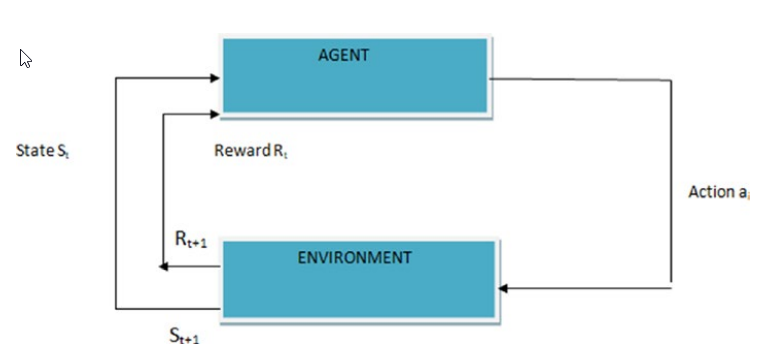
\includegraphics[scale=0.74]{ Reinforcement_Learning_interactions}
\caption{Reinforcement Learning interactions; }%from: \href{file:///H:/201906_fall/data/tmp/project2020-1/downloads/reinforcement_learning/2018_Book_ReinforcementLearning.pdf}{All the faces of Reinforcement Learning}
\end{center}
\end{figure}

The interactions between the agent and the environment occur with a reward. 
We need to take an action to move from one state to another.\\
Reinforcement Learning is a way of implementing how to map situations to actions 
so as to maximize and find a way to get the highest rewards.
The machine or robot is not told which actions to take, as with other forms of 
Machine Learning, but instead the machine must discover which actions yield the 
maximum reward by trying them.\\
%=----How Reward Works------------=%
\item How Reward Works\\
A reward is some motivator we receive when we transition from one state to another. It 
can be points, as in a video game. The more we train, the more accurate we become, and 
the greater our reward.\\
%=----Agents------------=%
\item Agents\\
In terms of Reinforcement Learning, agents are the software programs that make
intelligent decisions. Agents should be able to perceive what is happening in the
environment. Here are the basic steps of the agents:\\
\begin{itemize}
\item When the agent can perceive the environment, it can make
better decisions.
\end{itemize}
\begin{itemize}
\item The decision the agents take results in an action.
\end{itemize}
\begin{itemize}
\item The action that the agents perform must be the best, the
optimal, one.
\end{itemize}

\begin{figure}[hbt!]
\begin{center}
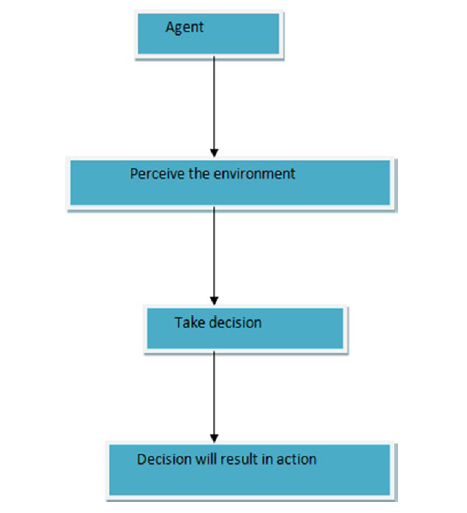
\includegraphics[scale=0.74]{agent}
\caption{agent}%from: \href{file:///H:/201906_fall/data/tmp/project2020-1/downloads/reinforcement_learning/2018_Book_ReinforcementLearning.pdf}{All the faces of Reinforcement Learning}
\end{center}
\end{figure}
%=----Agents------------=%
\item RL Environments\\
The environments in the Reinforcement Learning space are comprised of certain factors
that determine the impact on the Reinforcement Learning agent. The agent must adapt
accordingly to the environment. These environments can be 2D worlds or grids or even a 3D world.\\
\begin{large}
\textbf{Here are some important features of environments:}\end{large}\\
\begin{itemize}
\item Deterministic
\end{itemize}

\begin{itemize}
\item Observable
\end{itemize}
\begin{itemize}
\item Discrete or continuous
 
\end{itemize}
\begin{itemize}
\item Single or multiagent.
\end{itemize}
\end{itemize}
\newpage
\section{深度強化學習}
\subsection{Deep Reinforcement Learning}
\begin{figure}[hbt!]
\begin{center}
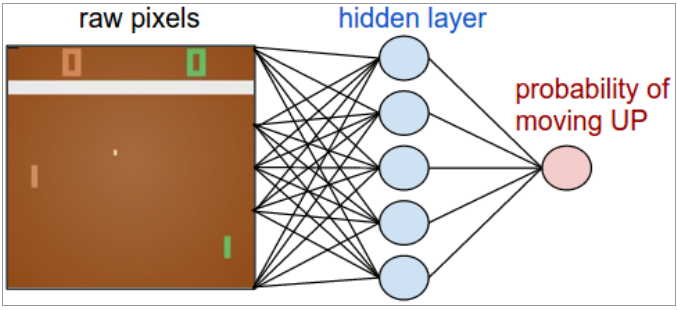
\includegraphics[scale=0.74]{ network}
\caption{Our network is a 2-layer fully-connected net. }%from: \href{file:///H:/201906_fall/data/tmp/project2020-1/downloads/reinforcement_learning/2018_Book_ReinforcementLearning.pdf}{All the faces of Reinforcement Learning}
\end{center}
\end{figure}\textbf{}

\qquad we're going to define a policy network that implements our player (or “agent”). This network will take the state of the game and decide what we should do (move UP or DOWN). As our favorite simple block of compute we'll use a 2-layer neural network that takes the raw image pixels (100,800 numbers total (210*160*3)), and produces a single number indicating the probability of going UP. Note that it is standard to use a stochastic policy, meaning that we only produce a probability of moving UP. Every iteration we will sample from this distribution (i.e. toss a biased coin) to get the actual move. The reason for this will become more clear once we talk about training.\\


\subsection{Supervised Learning}
\begin{figure}[hbt!]
\begin{center}
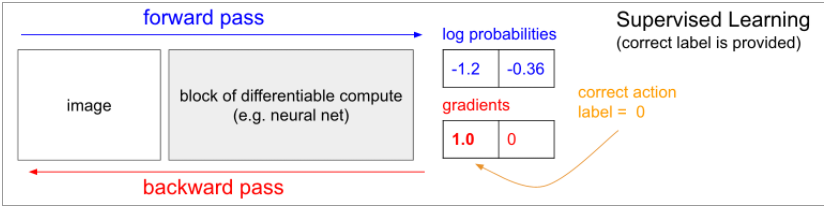
\includegraphics[scale=0.74]{supervising_learning}
\caption{supervising learning }%from: \href{file:///H:/201906_fall/data/tmp/project2020-1/downloads/reinforcement_learning/2018_Book_ReinforcementLearning.pdf}{All the faces of Reinforcement Learning}
\end{center}
\end{figure}
\textbf{}
Before we dive into the Policy Gradients solution I'd like to remind you briefly about supervised learning because, as we'll see, RL is very similar. Refer to the diagram below. In ordinary supervised learning we would feed an image to the network and get some probabilities, e.g. for two classes UP and DOWN. I'm showing log probabilities (-1.2, -0.36) for UP and DOWN instead of the raw probabilities (30 persent and 70 persent in this case) because we always optimize the log probability of the correct label (this makes math nicer, and is equivalent to optimizing the raw probability because log is monotonic). Now, in supervised learning we would have access to a label. For example, we might be told that the correct thing to do right now is to go UP (label 0). In an implementation we would enter gradient of 1.0 on the log probability of UP and run backprop to compute the gradient vector $Wlogp(y=UP|x)$. This gradient would tell us how we should change every one of our million parameters to make the network slightly more likely to predict UP. For example, one of the million parameters in the network might have a gradient of -2.1, which means that if we were to increase that parameter by a small positive amount (e.g. 0.001), the log probability of UP would decrease by 2.1 * 0.001 (decrease due to the negative sign). If we then did a parameter update then, our network would now be slightly more likely to predict UP when it sees a very similar image in the future.\\

\subsection{Log Derivative Trick}
\qquad 機器學習涉及操縱機率。這個機率通常包含normalised-probabilities或 log-probabilities。能加強解決現代機器學習問題的關鍵點,是能夠巧妙的在這兩種型式間交替使用,而對數導數技巧就能夠幫助我們做到這點,也就是運用對數導數的性質。\\
\subsection{Score Functions}
\qquad 對數導數技巧的應用規則是基於參數$\theta$梯度的對數函數$p(x:\theta)$,如下:\\
$$\nabla_\theta logp(x:\theta)=\frac{\nabla_\theta p(x:\theta)}{p(x:\theta)}$$\\
$p(x:\theta)$是likelihood ; function參數$\theta$的函數,它提供隨機變量x的概率。在此特例中,$\nabla_\theta logp(x:\theta)$被稱為Score Function,而上述方程式右邊為score ratio(得分比)。\\[6pt]

\begin{large}
{The score function has a number of useful properties:}
\end{large}
\begin{itemize}
\item The central computation for maximum likelihood estimation. Maximum likelihood is one of the dominant learning principles used in machine learning, used in generalised linear regression, deep learning, kernel machines, dimensionality reduction, and tensor decompositions, amongst many others, and the score appears in all these problems. 
\end{itemize}
\begin{itemize}
\item The expected value of the score is zero. Our first use of the log-derivative trick will be to show this.\\
$$\mathbb{E}_{p(x; \theta)}[\nabla_\theta \log p(\mathbf{x}; \theta)] =\mathbb{E}_{p(x; \theta)}\left[\frac{\nabla_\theta p(\mathbf {x}; \theta)}{p(\mathbf{x}; \theta)} \right]$$
$$= \int p(\mathbf {x}; \theta) \frac{\nabla_\theta p(\mathbf {x}; \theta)}{p(\mathbf{x}; \theta)} dx= \nabla_\theta \int p(\mathbf{x}; \theta) dx=\nabla_\theta 1 = 0$$\\
\qquad In the first line we applied the log derivative trick and in the second line we exchanged the order of differentiation and integration. This identity is the type of probabilistic flexibility we seek: it allows us to subtract any term from the score that has zero expectation, and this modification will leave the expected score unaffected (see control variates later).
\end{itemize}
\begin{itemize}
\item The variance of the score is the Fisher information and is used to determine the Cramer-Rao lower bound.\\
$$\mathbb{V}[\nabla_\theta \log p(\mathbf{x}; \theta)] = \mathcal{I}(\theta) =\mathbb{E}_{p(x; \theta)}[\nabla_\theta \log p(\mathbf{x}; \theta)\nabla_\theta \log p(\mathbf{x}; \theta)^\top]$$\\
We can now leap in a single bound from gradients of a log-probability to gradients of a probability, and back. But the villain of today's post is the troublesome expectation-gradient of Trick 4, re-emerged. We can use our new-found power—the score function—to develop yet another clever estimator for this class of problems.
\end{itemize}
\subsection{Score Function Estimators}
Our problem is to compute the gradient of an expectation of a function f:\\
$$\nabla_\theta \mathbb{E}_{p(z;\theta)}[f(z)] =\nabla_\theta \int p(z; \theta)f(z) dz$$\\

This is a recurring task in machine learning, needed for posterior computation in variational inference, value function and policy learning in reinforcement learning, derivative pricing in computational finance, and inventory control in operations research, amongst many others.

This gradient is difficult to compute because the integral is typically unknown and the parameters θ, with respect to which we are computing the gradient, are of the distribution p(z;θ). Furthermore, we might want to compute this gradient when the function f is not differentiable. Using the log derivative trick and the properties of the score function, we can compute this gradient in a more amenable way:\\
$$\nabla_\theta \mathbb{E}_{p(z;\theta)}[f(z)] = \mathbb{E}_{p(z;\theta)}[f(z)\nabla_\theta \log p(z;\theta)]$$\\
This is a recurring task in machine learning, needed for posterior computation in variational inference, value function and policy learning in reinforcement learning, derivative pricing in computational finance, and inventory control in operations research, amongst many others.

\qquad This gradient is difficult to compute because the integral is typically unknown and the parameters θ, with respect to which we are computing the gradient, are of the distribution p(z;θ). Furthermore, we might want to compute this gradient when the function f is not differentiable. Using the log derivative trick and the properties of the score function, we can compute this gradient in a more amenable way:\\
$$\nabla_\theta \mathbb{E}_{p(z;\theta)}[f(z)] = \mathbb{E}_{p(z;\theta)}[f(z)\nabla_\theta \log p(z;\theta)]$$\\
\begin{figure}[hbt!]
\begin{center}
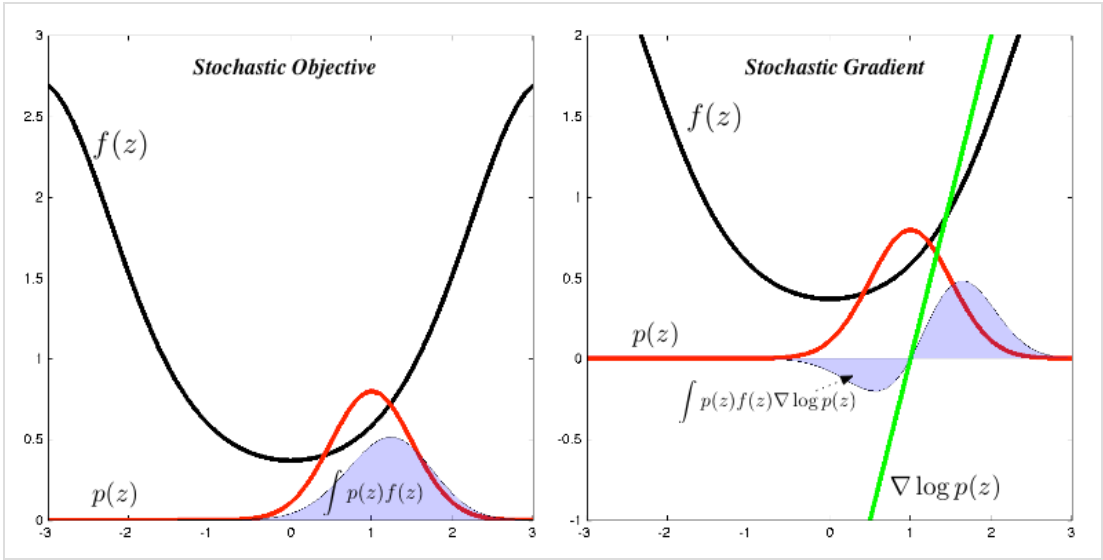
\includegraphics[scale=0.5]{gradient_change}
\caption{gradient change}%from: \href{file:///H:/201906_fall/data/tmp/project2020-1/downloads/reinforcement_learning/2018_Book_ReinforcementLearning.pdf}{All the faces of Reinforcement Learning}
\end{center}
\end{figure}
\qquad Let's derive this expression and explore the implications of it for our optimisation problem.\\
\qquad To do this, we are will use one other ubiquitous trick, a probabilistic identity trick, where we multiply our expressions by 1—a one formed by the division of a probability density by itself.  Combining the identity trick with the log-derivative trick, we obtain a score function estimator for the gradient:\\
$$\nabla_\theta \mathbb{E}_{p(z;\theta)}[f(z)]=\int\nabla_\theta p(z;\theta)f(z) dz$$\\[6pt]
$$= \int \frac{p(z;\theta)}{p(z;\theta)}\nabla_\theta p(z;\theta)f(z) dz$$\\[6pt]
$$=\int p(z;\theta)\nabla_\theta \log p(z;\theta)f(z) dz = \mathbb{E}_{p(z;\theta)}[f(z)\nabla_\theta \log p(z;\theta)]$$\\[6pt]
$$=\int p(z;\theta)\nabla_\theta \log p(z;\theta)f(z) dz = \mathbb{E}_{p(z;\theta)}[f(z)\nabla_\theta \log p(z;\theta)]$$\\[6pt]
$$\approx \frac{1}{S} \sum_{s=1}^{S}f(z^{(s)})\nabla_\theta \log p(z^{(s)};\theta) \quad z^{(s)}\sim p(z)$$\\[6pt]
A lot has happened in these four lines. In the first line we exchanged the derivative and the integral. In the second line, we applied our probabilistic identity trick, which allowed us to form the score ratio. Using the log-derivative trick, we then replaced this ratio with the gradient of the log-probability in the third line. This gives us our desired stochastic estimator in the fourth line, which we computed by Monte Carlo by first drawing samples from p(z) and then computing the weighted gradient term.\\

To put this in English, we have some distribution $p(x;\theta)$ (I used shorthand $p(x)$ to reduce clutter) that we can sample from (e.g. this could be a gaussian). For each sample we can also evaluate the score function f which takes the sample and gives us some scalar-valued score. This equation is telling us how we should shift the distribution (through its parameters θ) if we wanted its samples to achieve higher scores, as judged by f. In particular, it says that look: draw some samples x, evaluate their scores f(x), and for each x also evaluate the second term $\nabla_\theta logp(x;θ)$. What is this second term? It’s a vector - the gradient that’s giving us the direction in the parameter space that would lead to increase of the probability assigned to an x. In other words if we were to nudge θ in the direction of $\nabla_\theta logp(x;θ)$ we would see the new probability assigned to some x slightly increase. If you look back at the formula, it’s telling us that we should take this direction and multiply onto it the scalar-valued score $f(x)$. This will make it so that samples that have a higher score will “tug” on the probability density stronger than the samples that have lower score, so if we were to do an update based on several samples from p the probability density would shift around in the direction of higher scores, making highly-scoring samples more likely.
\begin{figure}[hbt!]
\begin{center}
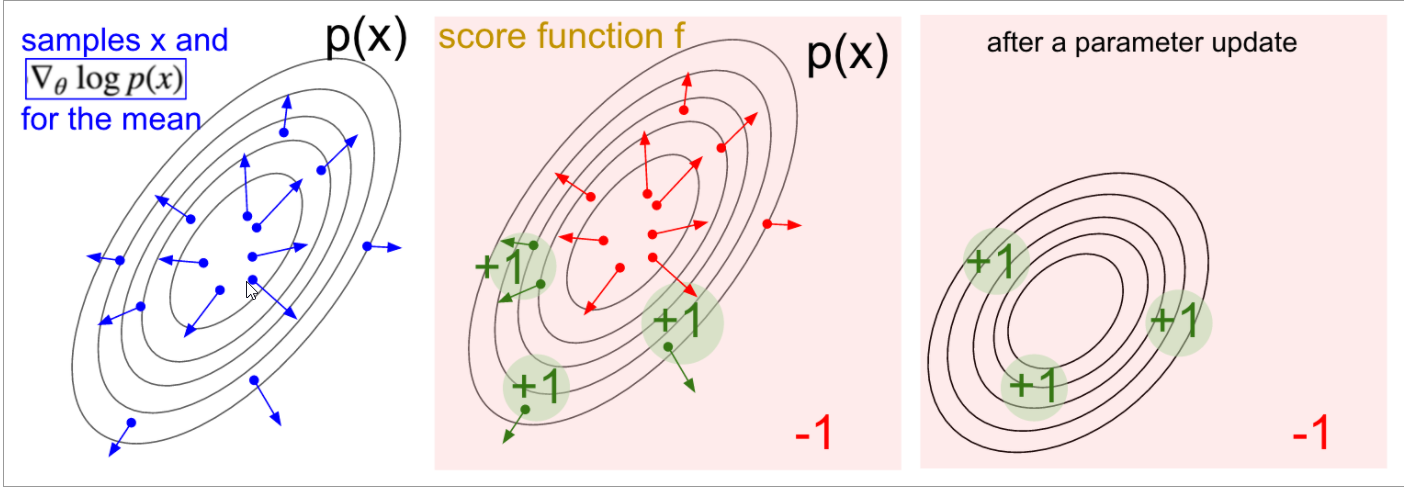
\includegraphics[scale=0.4]{figure}
%\caption{gradient change}%from: \href{file:///H:/201906_fall/data/tmp/project2020-1/downloads/reinforcement_learning/2018_Book_ReinforcementLearning.pdf}{All the faces of Reinforcement Learning}
\end{center}
\end{figure}
\qquad A visualization of the score function gradient estimator. Left: A gaussian distribution and a few samples from it (blue dots). On each blue dot we also plot the gradient of the log probability with respect to the gaussian's mean parameter. The arrow indicates the direction in which the mean of the distribution should be nudged to increase the probability of that sample. Middle: Overlay of some score function giving -1 everywhere except +1 in some small regions (note this can be an arbitrary and not necessarily differentiable scalar-valued function). The arrows are now color coded because due to the multiplication in the update we are going to average up all the green arrows, and the negative of the red arrows. Right: after parameter update, the green arrows and the reversed red arrows nudge us to left and towards the bottom. Samples from this distribution will now have a higher expected score, as desired.\\
\newpage
\section{比較個方法的特色}
\newpage
\chapter{優化器算法}
\section{Markov Decision Process}
\quad 在MRP中加入決策(decision)和動作(action)\\
\begin{itemize}
\item S:state 狀態
\item A:action 動作
\item P:狀態轉換\\[6pt]
\begin{center}
\hspace{-4em}\makebox[\width][s]{$P(s_{s+1}=s'|s_t=s,a_t=a)$}
\end{center}

\end{itemize}
\newpage
\chapter{訓練環境}
\section{openAI Gym}
\qquad Gym 是用於開發和比較強化學習算法的工具包,他不對agent的結構做任何假設,並且與任何數據計算庫兼容,而可以用來制定強化學習的算法。這個環境具有共享的介面,使我們能用來編寫常規算法,也就能教導agents如何步行到玩遊戲。\\[6pt]


\section{Pong}
\qquad 取自 1977年發行的一款家用遊戲機ATARI 2600中的遊戲,內建於Gym,這是一個橫向的乒乓遊戲,左方是遊玩者,右邊是馬可夫決策的特例,每個邊緣都會給予reward(figue1),目標就是計算再任意階段動作最佳路徑,已獲得rewardd最大值。
\section{Abstract}
\qquad I'd like to walk you through Policy Gradients (PG), our favorite default choice for attacking RL problems at the moment. If you’re from outside of RL you might be curious why I’m not presenting DQN instead, which is an alternative and better-known RL algorithm, widely popularized by the ATARI game playing paper. It turns out that Q-Learning is not a great algorithm (you could say that DQN is so 2013 . In fact most people prefer to use Policy Gradients, including the authors of the original DQN paper who have shown Policy Gradients to work better than Q Learning when tuned well. PG is preferred because it is end-to-end: there's an explicit policy and a principled approach that directly optimizes the expected reward. Anyway, as a running example we'll learn to play an ATARI game (Pong!) with PG, from scratch, from pixels, with a deep neural network, and the whole thing is 130 lines of Python only using numpy as a dependency (Gist link). Lets get to it.

\section{Pong from pixels}
\qquad Left: The game of Pong. Right: Pong is a special case of a Markov Decision Process (MDP): A graph where each node is a particular game state and each edge is a possible (in general probabilistic) transition. Each edge also gives a reward, and the goal is to compute the optimal way of acting in any state to maximize rewards.\\ 
The game of Pong is an excellent example of a simple RL task. In the ATARI 2600 version we’ll use you play as one of the paddles (the other is controlled by a decent AI) and you have to bounce the ball past the other player (I don’t really have to explain Pong, right?). On the low level the game works as follows: we receive an image frame (a 210x160x3 byte array (integers from 0 to 255 giving pixel values)) and we get to decide if we want to move the paddle UP or DOWN (i.e. a binary choice). After every single choice the game simulator executes the action and gives us a reward: Either a +1 reward if the ball went past the opponent, a -1 reward if we missed the ball, or 0 otherwise. And of course, our goal is to move the paddle so that we get lots of reward.\\

\newpage
\chapter{模擬環境}
\newpage
\chapter{伺服器}
\begin{itemize}
\item Oracle VM VirtualBox\\
\qquad 因應在虛實整合需要用到虛擬環境去模擬的情況,我們使用 Ubuntu 當作我們的作業系統去建構虛擬環境,而在此之前要先安裝「虛擬機器工作站」— Oracle VM VirtualBox 。
\section{Oracle VM VirtualBox 介紹}
當要使用不同的的作業系統 ( Linux , Ubuntu , Red Hat ...  ) 而不想與其資料存放時共用一個硬碟 ( 沒有多餘硬碟 , 不想硬碟之間有資料重疊 ... ) 時,就可以使用其軟體做練習,降低操作失誤帶來的成本,而此軟體目前為免費,並隨時會更新,另外其特色有 :
\item 只要自備作業系統 ( 光碟片 , ISO映像檔 ) ,即可在啟動 Oracle VM VirtualBox  後直接開啟要操作的執行檔 ( 作業系統 ),不必再把主機本身重新關機,當然開啟多個作業系統之間也有共通性,可直接從視窗A做網路、檔案分享、複製貼上等動作到視窗B。
\item 除了作業系統裡面的執行,還可在其中練習磁碟分割、格式化以及 BIOS 啟動等 ( 但是未支援USB啟動 ) 。
\item 空間的佔用上並不是真實佔用空間,而是依據使用者的操作而變化 ( 使用者用多少就是多少 )。相對的,使用者雖然一開始設定該虛擬電腦的記憶體大小與硬碟空間是實時依據操作者決定,但終究還是佔掉電腦效能,所以 VirtualBox 的效能還是依據電腦本身的硬體配備
\item
\end{itemize}
\newpage
\chapter{深度強化學習的訓練與控制}
\newpage
\chapter{問題與討論}

%=---------------------參考文獻----------------------=%
\newpage
\begin{center}
\addcontentsline{toc}{chapter}{參考文獻 }
\LARGE\textbf 參考文獻\\
\end{center}
\begin{flushleft}
\begin{Large}
[1]\quad https://towardsdatascience.com/derivative-of-the-sigmoid-function-536880cf918e\\

[2]\quad https://towardsdatascience.com/adam-latest-trends-in-deep-learning-optimization-6be9a291375c\\
\end{Large}
\end{flushleft}
\newpage
\begin{center}
\LARGE\textbf 作者簡介\\
\end{center}

\framebox[8cm][r]{\vspace{1em}test}


\end{document}
